\documentclass[a4paper,12pt]{article}
\usepackage[warn]{mathtext}
\usepackage[english, russian]{babel}
\usepackage[utf8]{inputenc}
\usepackage[letterpaper,top=2cm,bottom=2cm,left=3cm,right=3cm,marginparwidth=1.75cm]{geometry}
\usepackage{amsmath}
\usepackage{graphicx}
\graphicspath{{pictures/}}
\DeclareGraphicsExtensions{.jpg}
\DeclareGraphicsExtensions{.png}
\usepackage[colorlinks=true, allcolors=blue]{hyperref}
\usepackage{minted}
\usepackage{listings}
\usepackage{color}
\usepackage{mathtools}
\DeclarePairedDelimiter\ket{\lvert}{\rangle}

\title{Домашняя работа №3}
\author{A-05-19 Карпов Денис}
\date{}

\begin{document}
\maketitle

\section*{2. Машины Тьюринга}

\subsection*{2.1 Операции с языками и символами}

\text{Сложение двух унарных чисел (1 балл)}
 \begin{minted}[]{yaml}
            # 2_1_1.yaml
            input: '111+1'
            blank: ' '
            start state: right
            table:
              right:
                1: R
                '+': {write: '1', R: tail}
              tail:
                1: R
                ' ': {L: del_and_return}
              del_and_return:
                1: {write: ' ', L: return}
              return:
                1: L
                ' ': {R: done}
              done:
        \end{minted}
        \begin{center}
            \includegraphics[width=0.6\textwidth]{2_1_1.jpg} \\
        \end{center}
        
\text{Умножение унарных чисел}

 \begin{minted}[]{yaml}
            # 2_1_2.yaml
           input: '1111*11'
            blank: ' '
            start state: q0
            table:
              q0:
                1: R
                '*': {R: q1}
              q1:
                1: R
                ' ': {write: '=', L: q2}
              q2:
                1: {write: '0', L: q3}
              q3:
                1: L
                '*': L
                0: L
                '=': L
                ' ': {R: q4}
                'x': {R: q4}
              q4:
                1: {write: 'x', R: q5}
                '*': {L: q6}
              q5:
                0: R 
                1: R 
                '*': R
                '=': R
                ' ': {write: '1', L: q3}
              q6:
                'x': {write: 1, L}
                ' ': {R: q7}
              q7:
                1: R
                '*': R
                0: R
                '=': {L: q8}
              q8:
                0: L
                1: {write: '0', L: q3}
                '*': {R: q9}
              q9:
                0: {write: '1', R}
                '=':  {R: end}
              end:
        \end{minted}
        \begin{center}
            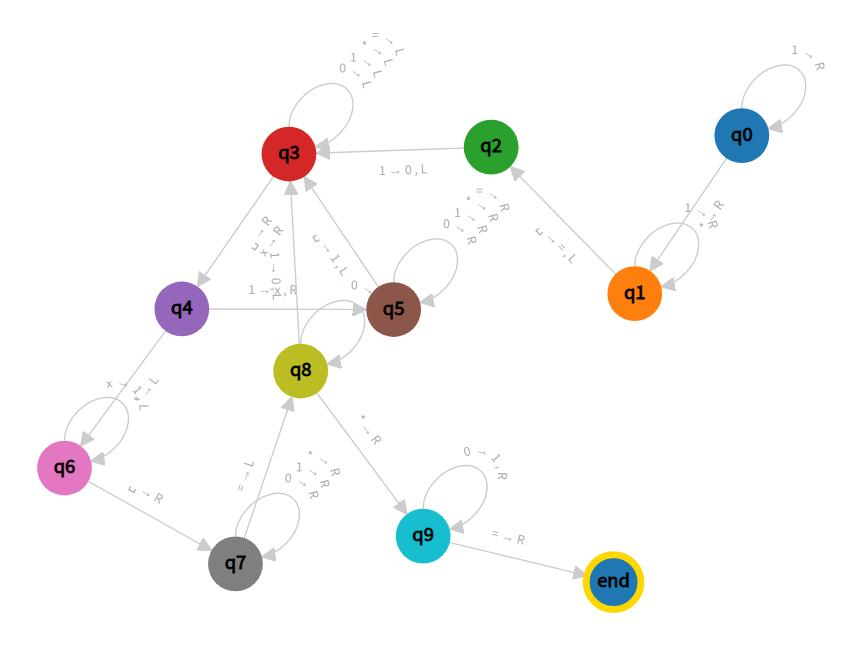
\includegraphics[width=\textwidth]{2_1_2.jpg} \\
        \end{center}
        
        \subsection*{2.2 Операции с языками и символами}
        Реализуйте машины Тьюринга, которые позволяют выполнять следующие операции:\newline
        1.Принадлежность к языку $L = \{ 0^n1^n2^n \}, n \ge 0$ (0.5 балла)\newline
        \begin{itemize}
            \item Выводит 'T', если слово принадлежит языку.
            \item Выводит 'F', если слово не принадлежит языку.
        \end{itemize}
        \begin{minted}[]{yaml}
            # 2_2_1.yaml
            input: '000111222'
            blank: ' '
            start state: newstart
            table:
              newstart:
                0: L
                ' ': {write: 's', R: start}
              start:
                0: {write: 'a', R: q0}
                a: R
                [b, c, 1, 2]: {R: bad}
                ' ': {write: 'T', L: end}
              q0:
                0: R
                1: {write: 'b', R: q1}
                b: R
                [a, c, 2]: {R: bad}
                ' ': {write: 'F', L: end}
              q1:
                1: R
                2: {write: 'c', R: q2}
                c: R
                [a, b, 0]: {R: bad}
                ' ': {write: 'F', L: end}
              q2:
                [0, 1, 2, 'a', 'b', 'c']: L
                s: {R: start}
                ' ': {L: rerun}
              rerun:
                [a, b, c]: L
                [0, 1, 2]: {R: bad}
                s: {R: good}
              bad:
                [0, 1, 2, 'a', 'b', 'c']: R
                ' ': {write: 'F', L: end}
              good:
                [0, 1, 2, 'a', 'b', 'c']: R
                ' ': {write: 'T', L: end}
              end:
    

        \end{minted}
        \begin{center}
            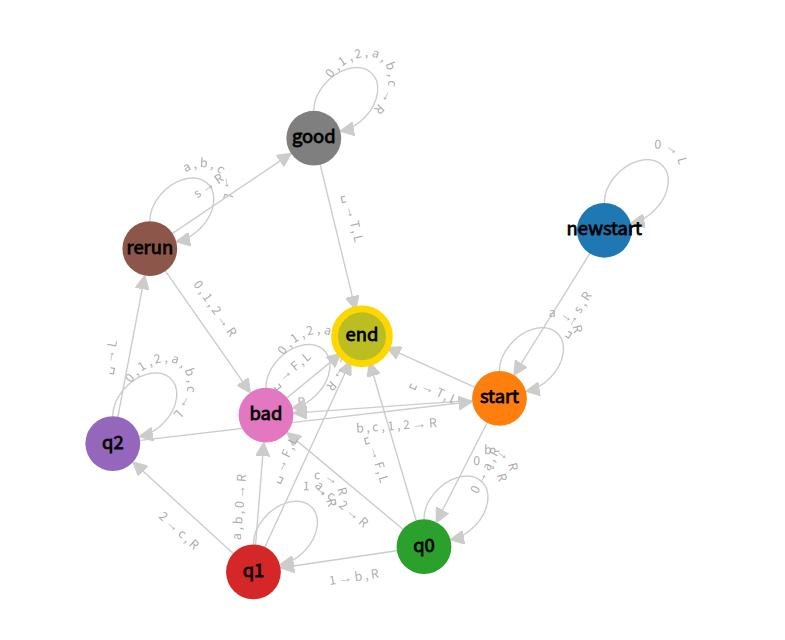
\includegraphics[width=\textwidth]{2_2_1.jpg} \\
        \end{center}
        Проверка соблюдения правильности скобок в строке (минимум 3 вида скобок) (0.5 балла)
        \begin{minted}[]{yaml}
            # 2_2_2.yaml
            input: '([{}])'
            blank: ' '
          start state: start
          table:
            start:
              ' ': {L: ok}    # пустая скобочная послед
              ['(', '[', '{']: {R: find-closed}
              [')', ']', '}']: {L: not-ok}
              
            find-closed:
              ' ': {L: empty-or-ok}    # вышли за граицы слова или не нашли закрывающуюся скобку
              ['(', '[', '{', 'x']: R
              ')': {write: 'x', L: closed_1}
              ']': {write: 'x', L: closed_2}
              '}': {write: 'x', L: closed_3}
            
            closed_1:
              ' ': {R: not-ok}
              '(': {write: 'x', R:  find-closed}
              ['[', '{']: {L: not-ok}
              'x': L
            
            closed_2:
              ' ': {R: not-ok}
              '[': {write: 'x', R: find-closed}
              ['(', '{']: {L: not-ok}
              'x': L
            
            closed_3:
              ' ': {R: not-ok}
              '{': {write: 'x', R: find-closed}
              ['[', '(']: {L: not-ok}
              'x': L 
              
            empty-or-ok:
              ['(', '[', '{']: {L: not-ok} # всё-таки есть необработанная скобка
              'x': L
              ' ': {R: ok}
              
            not-ok:
              ['(', ')', '[', ']', '{', '}', 'x']: {write: ' ', R}
              ' ': {R: go-start}
            # в начало, чтобы очистить ленту
            go-start:
              ['(', ')', '[', ']', '{', '}', 'x']: {write: ' ', R: go-start}
              ' ': {write: 0, L: done}
              
            ok:
              ' ': {write: 1, L: done}
              'x': {write: ' ', R}
            
            done:
    
        \end{minted}
        \begin{center}
            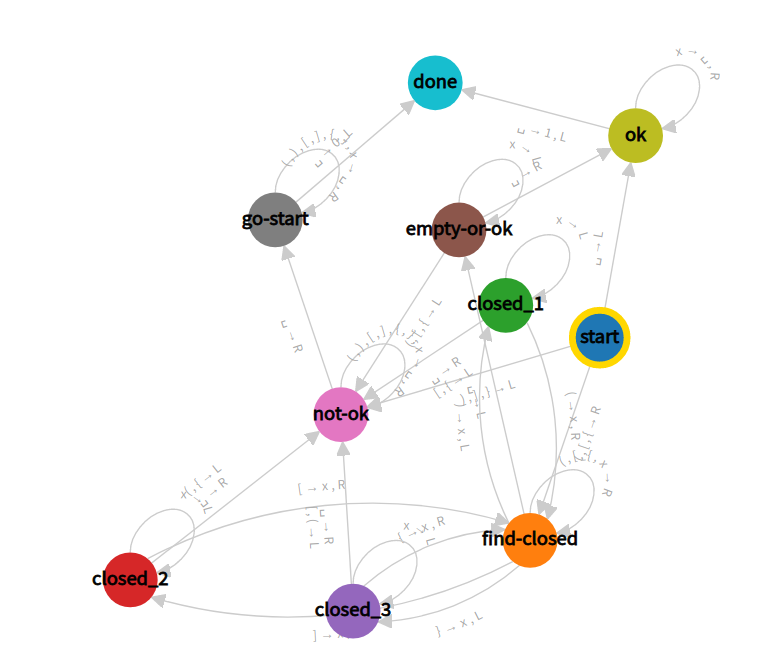
\includegraphics[width=\textwidth]{2_2_2} \\
        \end{center}
        
        Поиск минимального по длине слова в строке (слова состоят из символов 1 и 0 и разделены пробелом)
        \begin{minted}[]{yaml}
            # 2_2_3.yaml
            input: 'l110 01 11l'
            blank: ' '
            start state: start
            table:
              start:
                0: {write: 'a', R: q0}
                1: {write: 'b', R: q0}
                ['a', 'b', 'l']: R
                ' ': {write: '+', L: end}
                
              # один раз заменяем за проход
              q0:
                [0, 1, 'a','b']: R
                'l': {write: 'l', L: q1} # разворачиваемся
                ' ': {write: ' ', R: start}
                  
              q1:
                ['a','b', ' ']: L
                0: {write: 'a', L: q2}
                1: {write: 'b', L: q2}
                'l': {write: 'l', R: q2}
              
              q2:
                [0, 1, 'a','b']: L
                ' ': {write: ' ', L: q1}
                'l': {write: 'l', R: start}
              
              end:
                ['y','l']: L
                'a': {write: '0', L}
                'b': {write: '1', L}
                ' ': {write: ' ', R: done}
                
              done:
    
        \end{minted}
        \begin{center}
            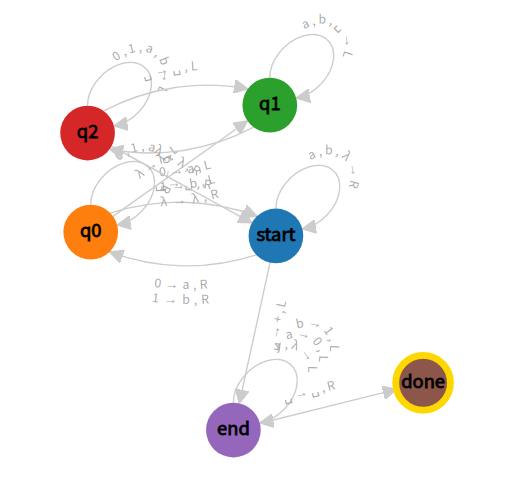
\includegraphics[width=\textwidth]{2_2_3} \\
        \end{center}
        
    \section*{3 Квантовые вычисления}
    \subsection*{3.1 Генерация суперпозиций 1 (1 балл)}
     Дано $N$ кубитов ($1 \le N \le 8$) в нулевом состоянии $\ket{0\dots0}$. 
    Также дана некоторая последовательность битов, которое задаёт ненулевое базисное состояние размера $N$. Задача получить суперпозицию нулевого состояния и заданного.
    
    $$\ket{S} = \frac{1}{\sqrt2}(\ket{0\dots0} +\ket{\psi})$$
    
    То есть, требуется реализовать операцию, которая принимает на вход:
    \begin{enumerate}
        \item Массив кубитов $q_s$
        \item Массив битов $bits$ описывающих некоторое состояние $\ket{\psi}$. Это массив имеет тот же самый размер, что и $q_s$. Первый элемент этого массива равен $1$.
    \end{enumerate}
    \textbf{Код}
    
    \begin{lstlisting}
        namespace Solution {
            open Microsoft.Quantum.Primitive;
            open Microsoft.Quantum.Canon;
            operation Solve (qs : Qubit[], bits : Bool[]) : Unit 
            {
                body
                {
                    H(qs[0]);
                    for i in 1..Length(qs) - 1 {
                        if (bits[i]) {
                            CNOT(qs[0], qs[i]);
                        }
                    }
                }
            }
        }
    \end{lstlisting}
    
    \subsection*{3.2 Различение состояний 1 (1 балл)}

    Дано $N$ кубитов ($1 \le N \le 8$), которые могут быть в одном из двух состояний:
    
    $$\ket{GHZ} = \frac{1}{\sqrt2}(\ket{0\dots0} +\ket{1\dots1})$$
    $$\ket{W} = \frac{1}{\sqrt N}(\ket{10\dots00}+\ket{01\dots00} + \dots +\ket{00\dots01})$$
    
    Требуется выполнить необходимые преобразования, чтобы точно различить эти два состояния. Возвращать $0$, если первое состояние и 1, если второе. 
    
    \textbf{Код}

    \begin{lstlisting}
        namespace Solution {
            open Microsoft.Quantum.Primitive;
            open Microsoft.Quantum.Canon;
            operation Solve (qs : Qubit[]) : Int 
            {
                body
                {
                    mutable ones = 0;
                    for i in 0..Length(qs) - 1 {
                        if (M(qs[i]) == One) {  // measurement
                            set ones += 1;
                        }
                    }
                    if (ones == 1) {
                        return 1;
                    }
                    return 0;
                }
            }
        }
    \end{lstlisting}
 
    
\newpage

\end{document}
